\section{Izhikevich モデル}
\subsection{Izhikevich モデルの定義}
\textbf{Izhikevich モデル}\index{Izhikevich もでる@Izhikevich モデル} (または\textbf{Simple model}\index{Simple model})はHHモデルとLIFモデルの中間のようなモデルである{cite;p}\jl{Izhikevich2003-by}.HHモデルのような生理学的な知見に基づいたモデルは実際のニューロンの発火特性をよく再現できるが,式が複雑化するため,数学的な解析が難しく,計算量が増えるために大規模なシミュレーションも困難となる\footnote{これに関しては必ずしも正しくない.計算機の発達によりHHモデルで大きなモデルをシミュレーションすることも可能である.}.そこで,生理学的な正しさには目をつぶり,生体内でのニューロンの発火特性を再現するモデルが求められた.その特徴を持つのがIzhikevich モデルである (以下ではIzモデルと表記する).Izモデルは 2変数しかない\footnote{数値計算をする上では簡易的だが,if文が入るために解析をするのは難しくなる.([Bernardo, et al., 2008](https://www.springer.com/gp/book/9781846280399))\url{http://www.scholarpedia.org/article/Piecewise_smooth_dynamical_systems}を読むといいらしい.}
簡素な微分方程式だが, 様々なニューロンの活動を模倣することができる\citep{Izhikevich2004-xf}.定式化には主に2種類ある.まず,{cite;p}\jl{Izhikevich2003-by}で提案されたのが次式である.
\begin{align}
\frac{dv(t)}{dt}&=0.04v(t)^2 + 5v(t)+140-u(t)+I(t) \\
\frac{du(t)}{dt}&=a(bv(t)-u(t))
\end{align} 
ここで,$v$と$u$が変数であり, $v$は膜電位(membrane potential;単位はmV), $u$は回復電流(recovery current; 単位はpA)\footnote{ここでの「回復」というのは脱分極した後の膜電位が静止膜電位へと戻る,という意味である (対義語はactivationで膜電位の上昇を意味する).$u$は$v$の導関数において$v$の上昇を抑制するように$-u$で入っているため,$u$としてはK$^+$チャネル電流やNa$^+$チャネルの不活性化動態などが考えられる.}
である.また,$a$は回復時定数(recovery time constant; 単位はms$^{-1}$)の逆数 (これが大きいと$u$が元に戻る時間が短くなる), $b$は$u$の$v$に対する感受性(共鳴度合い,  resonance; 単位はpA/mV)である.
この式は簡便だが,生理学的な意味づけが分かりにくい.改善された式として\citep{Izhikevich2007-ff}のChapter 8で紹介されているのが次式である.
\begin{align}
C\frac{dv(t)}{dt}&=k\left(v(t)-v_r\right)\left(v(t)-v_t\right)-u(t)+I(t) \\
\frac{du(t)}{dt}&=a\left\{b\left(v(t)-v_{r}\right)-u(t)\right\}
\end{align} 
ここで,$C$は膜容量(membrane capacitance; 単位はpF), $v_r$は静止膜電位(resting membrane potential; 単位はmV), $v_t$は閾値電位(instantaneous threshold potential; 単位はmV), $k$はニューロンのゲインに関わる定数で,小さいと発火しやすくなる (単位はpA/mV).以後はこちらの式を用いる.
Izモデルの閾値の取り扱いはLIFモデルと異なり,HHモデルに近い.LIFモデルでは閾値を超えた時に膜電位をピーク電位まで上昇させ (この過程は無くてもよい),続いて膜電位をリセットする.Izモデルの閾値は$v_t$だが, 膜電位のリセットは閾値を超えたかで判断せず,膜電位$v$がピーク電位$v_{\text{peak}}$になったとき (または超えた時) に行う.そのためIzモデルの実際の閾値は膜電位の挙動が変化する(発火状態に移行する),つまり分岐(bifurcation) が生じる点であり,パラメータの閾値$v_t$との間には差異がある.
さて,膜電位がピーク電位$v_{\text{peak}}$に達したとき (すなわち \jl{if} $v \geq v_{\text{peak}}$),$u, v$を次のようにリセットする\footnote{バースト発火(bursting)の挙動を表現するためには,速い回復変数(fast recovery variable)と遅い回復変数(slow recovery variable)の2つが必要となる(従って膜電位も合わせて全部で3変数必要).一方で,IzモデルではLIFモデルのようなif文によるリセットを用いているため,速い回復変数が必要なく,遅い回復変数$u$のみでバースト発火を表現できる.}.
\begin{align} 
u&\leftarrow u+d\\
v&\leftarrow v_{\text{reset}}
\end{align}
とする.ただし, $v_{\text{reset}}$は過分極を考慮して静止膜電位$v_r$よりも小さい値とする.また,$d$はスパイク発火中に活性化される正味の外向き電流の合計を表し,発火後の膜電位の挙動に影響する (単位はpA).
以上を踏まえて, シミュレーションを行う.まず,必要なパッケージを読み込む.
\begin{lstlisting}[language=julia]
using Parameters: @unpack # or using UnPack
using PyPlot
rc("axes.spines", top=false, right=false)
\end{lstlisting}
変更しない定数を保持する\jl{struct}の\jl{IZParameter}と,変数を保持する\jl{mutable struct}の\jl{IZ}を作成する.2つの定式化でパラメータの値が異なるので注意すること.
\begin{lstlisting}[language=julia]
@kwdef struct IZParameter{FT}
    C::FT = 100  # 膜容量 (pF)
    a::FT = 0.03; b::FT = -2 # 回復時定数の逆数 (1/ms), uのvに対する共鳴度合い (pA/mV)
    d::FT = 100; k::FT = 0.7 # 発火で活性化される正味の外向き電流 (pA), ゲイン (pA/mV)
    vthr::FT = -40; vrest::FT = -60; vreset::FT = -50; vpeak::FT = 35 # 閾値電位, 静止膜電位, リセット電位, ピーク電位 (mV)
end

@kwdef mutable struct IZ{FT}
    param::IZParameter = IZParameter{FT}()
    N::UInt32
    v::Vector{FT} = fill(param.vrest, N); u::Vector{FT} = zeros(N)
    fire::Vector{Bool} = zeros(Bool, N)
end
\end{lstlisting}
次に変数を更新する関数\jl{update!}を書く.LIFの場合と異なり,\jl{v[i] >= vpeak}であることに注意する (\jl{v[i] >= vthr}ではない).
\begin{lstlisting}[language=julia]
function update!(variable::IZ, param::IZParameter, Ie::Vector, dt)
    @unpack N, v, u, fire = variable
    @unpack C, a, b, d, k, vthr, vrest, vreset, vpeak = param
    @inbounds for i = 1:N
        v[i] += dt/C * (k*(v[i]-vrest)*(v[i]-vthr) - u[i] + Ie[i])
        u[i] += dt * (a * (b * (v[i]-vrest) - u[i]))
    end
    @inbounds for i = 1:N
        fire[i] = v[i] >= vpeak
        v[i] = ifelse(fire[i], vreset, v[i])
        u[i] += ifelse(fire[i], d, 0)
    end
end;
\end{lstlisting}
\subsection{Izhikevich モデルのシミュレーションの実行}
いくつかの定数を設定してシミュレーションを実行する.
\begin{lstlisting}[language=julia]
T = 450 # ms
dt = 0.01f0 # ms
nt = UInt32(T/dt) # number of timesteps
N = 1 # ニューロンの数

# 入力刺激
t = Array{Float32}(1:nt)*dt
Ie = repeat(150f0 * ((t .> 50) - (t .> 200)) + 300f0 * ((t .> 250) - (t .> 400)), 1, N)  # injection current

# 記録用
varr, uarr = zeros(Float32, nt, N), zeros(Float32, nt, N)

# modelの定義
neurons = IZ{Float32}(N=N)

# simulation
@time for i = 1:nt
    update!(neurons, neurons.param, Ie[i, :], dt)
    varr[i, :], uarr[i, :] = neurons.v, neurons.u
end
\end{lstlisting}
\jl{Plots}を読み込み,膜電位\jl{v}, 回復変数\jl{u}, 入力電流\jl{I}を描画する.
\begin{lstlisting}[language=julia]
figure(figsize=(4, 4))
suptitle("Regular Spiking (RS) Neurons")
subplot(3,1,1); plot(t, varr[:, 1]); ylabel("Membrane\n potential (mV)")
subplot(3,1,2); plot(t, uarr[:, 1]); ylabel("Recovery\n current (pA)")
subplot(3,1,3); plot(t, Ie[:, 1]); ylabel("Injection\n current (pA)"); xlabel("Times (ms)")
tight_layout(rect=[0,0,1,0.96])
\end{lstlisting}
\begin{figure}[ht]
	\centering
	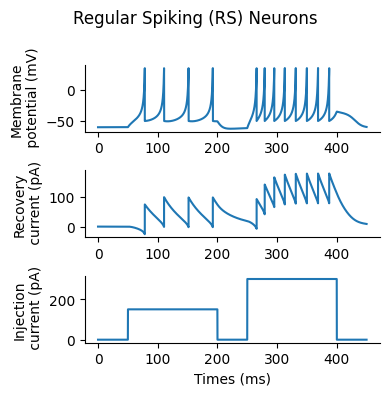
\includegraphics[scale=0.8, max width=\linewidth]{./fig/neuron-model/izhikevich/cell009.png}
	\caption{cell009.png}
	\label{cell009.png}
\end{figure}
\subsection{様々な発火パターンのシミュレーション}
次に様々な発火パターンを模倣するようにIzモデルの定数を変化させてみよう.Intrinsically Bursting (IB)ニューロンとChattering (CH) ニューロン(または fast rhythmic bursting (FRB) ニューロン)のシミュレーションを行う.基本的には定数を変えるだけである.
本書で用いている式における発火パターンに対するパラメータは{cite;p}\jl{Izhikevich2003-by}では得られないが,\citep{Izhikevich2007-ff}には記載がある.他の発火パターンに関してはこの本を参照のこと.
\begin{lstlisting}[language=julia]
# 記録用
varr_ib, varr_ch = zeros(Float32, nt, N), zeros(Float32, nt, N)
Ie = repeat(500f0 * ((t .> 50) - (t .> 200)) + 700f0 * ((t .> 250) - (t .> 400)), 1, N)  # injection current

# IB neurons
neurons_ib = IZ{Float32}(N=N, 
    param=IZParameter{Float32}(C = 150, a = 0.01, b = 5, k =1.2, d = 130, vrest = -75, vreset = -56, vthr = -45, vpeak = 50))

# CH neurons
neurons_ch = IZ{Float32}(N=N, 
    param=IZParameter{Float32}(C = 50, a = 0.03, b = 1, k =1.5, d = 150, vrest = -60, vreset = -40, vthr = -40, vpeak = 35))

# simulation
@time for i = 1:nt
    update!(neurons_ib, neurons_ib.param, Ie[i, :], dt)
    update!(neurons_ch, neurons_ch.param, Ie[i, :], dt)
    varr_ib[i, :], varr_ch[i, :] = neurons_ib.v, neurons_ch.v
end
\end{lstlisting}
これまでと異なり,モデルの定義時に\jl{param}を設定していることに注意しよう.最後に膜電位変化を描画する.
\begin{lstlisting}[language=julia]
figure(figsize=(6, 2))
subplot(1,2,1); plot(t, varr_ib[:, 1]); title("IB Neurons"); ylabel("Membrane\n potential (mV)");  xlabel("Times (ms)")
subplot(1,2,2); plot(t, varr_ch[:, 1]); title("CH neurons"); xlabel("Times (ms)")
tight_layout()
\end{lstlisting}
\begin{figure}[ht]
	\centering
	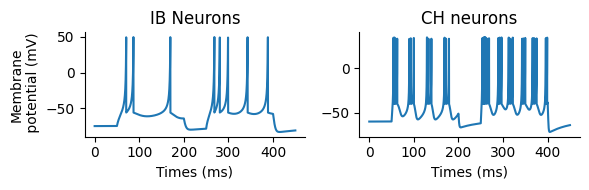
\includegraphics[scale=0.8, max width=\linewidth]{./fig/neuron-model/izhikevich/cell013.png}
	\caption{cell013.png}
	\label{cell013.png}
\end{figure}
